\documentclass[a4paper,11pt]{article}
%\documentclass[11pt,twocolumn]{article}
\usepackage[utf8]{inputenc}
\usepackage{graphicx}

\begin{document}
	\author{
	Aveiga Iván \ Enriquez Wilson \ Sornoza Andrés
	}
\title{Notify Me}
\maketitle
\begin{figure}[h]
\centering

\includegraphics[width=0.7\linewidth]{./logo}
\end{figure}

\vspace{7mm}

NotifyMe es una aplicación que servirá de servicio de recordatorios (\emph{to do}) que añade la funcionalidad de ubicación geográfica. Solucionando el problema de que usuarios de otras aplicaciones de tipo \emph{to do} no lograban realizar las tareas especificadas ya que eran simples recordatorios. \\

NotifyMe se diferencia de estas aplicaciones en que a la nota o tare a realizar se añade un lugar geográfico, esto ayuda que en cuando el usuario esté en un rango (escogido por el usuario)de dicha ubicación determinada previamente emite una alarma para que el usuario realice la actividad anotada.

\section{\textbf{Detalles técnicos:}}
A continuación podemos ver el diagrama de casos de uso de la NotifyMe \\
\begin{figure}[h]
\centering
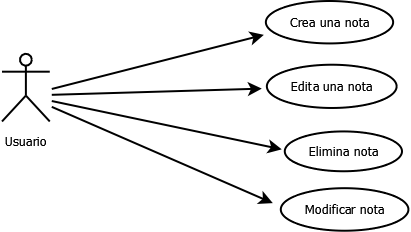
\includegraphics[width=0.7\linewidth]{./CasoDeUso}
\end{figure}


NotifyMe usa el \emph{GPS} del smartphone para poder ubicar la posición actual del usuario, y por medio de la \emph{API de Google Maps} poder ubicar el lugar geográfico de la nota o tarea a realizar. Se usa de una base de datos de \emph{SQLite}d e una sola tabla que contiene datos como tarea, ubicación geográfica, categoría, si se realizó la tarea, esto con el fin de recolectar datos y en futuras versiones ofrecer historiales de tareas realizadas, tareas no realizadas, tareas agrupadas por lugares geográficos o categorías. \\
 
Modelo de Base de Datos: \\

Dada que la aplicación es sencilla, solo se cuenta con dos tablas: \\

\begin{figure}[h]
\centering
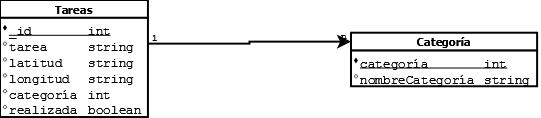
\includegraphics[width=0.7\linewidth]{./DB}
\caption{}
\label{fig 1: Modelo ER de Base de Datos de NotifyMe}
\end{figure}

NotifyMe será implementado para Smartphones que tengan el Sistema Operativo Android 2.3.6 (\emph{Gingerbread}) o superior. Como lenguaje de programación se usa Java, y para persistencia de datos SQLite que se encuentra embebido en Android.
\end{document}